
\section*{Appendix \hypertarget{AppA:Figures}{A}: Figures} \label{App:Figures}

\subsection*{\hypertarget{AppA1:Figures:Excludedc}{A1} Excluded consumer data sets}\label{AppA1:Figures:Excludedc}

\begin{centering}
\begin{figure}[!htbp]
        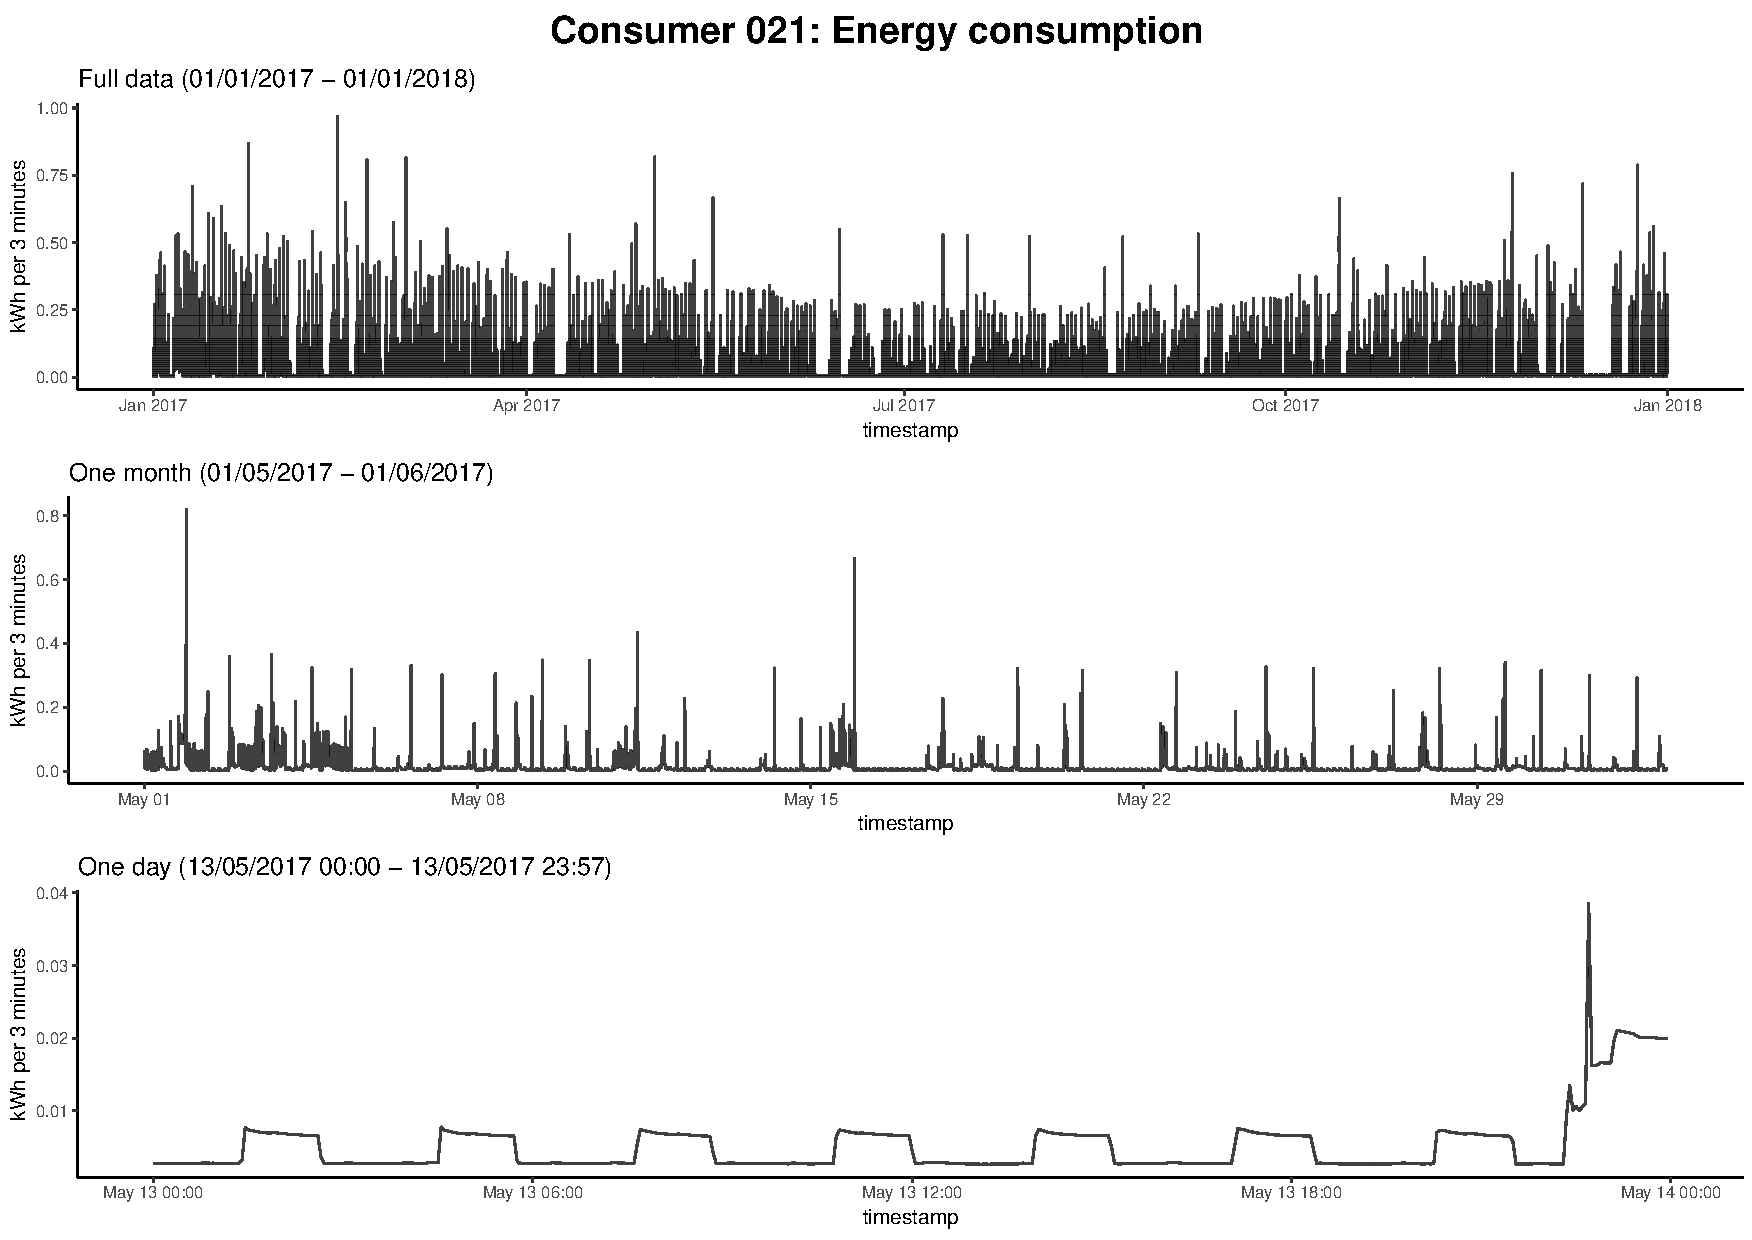
\includegraphics[width=\textwidth-0.85cm]{thesis/graphs/timeseries/c021_cons.pdf}\vspace{0.3cm}
        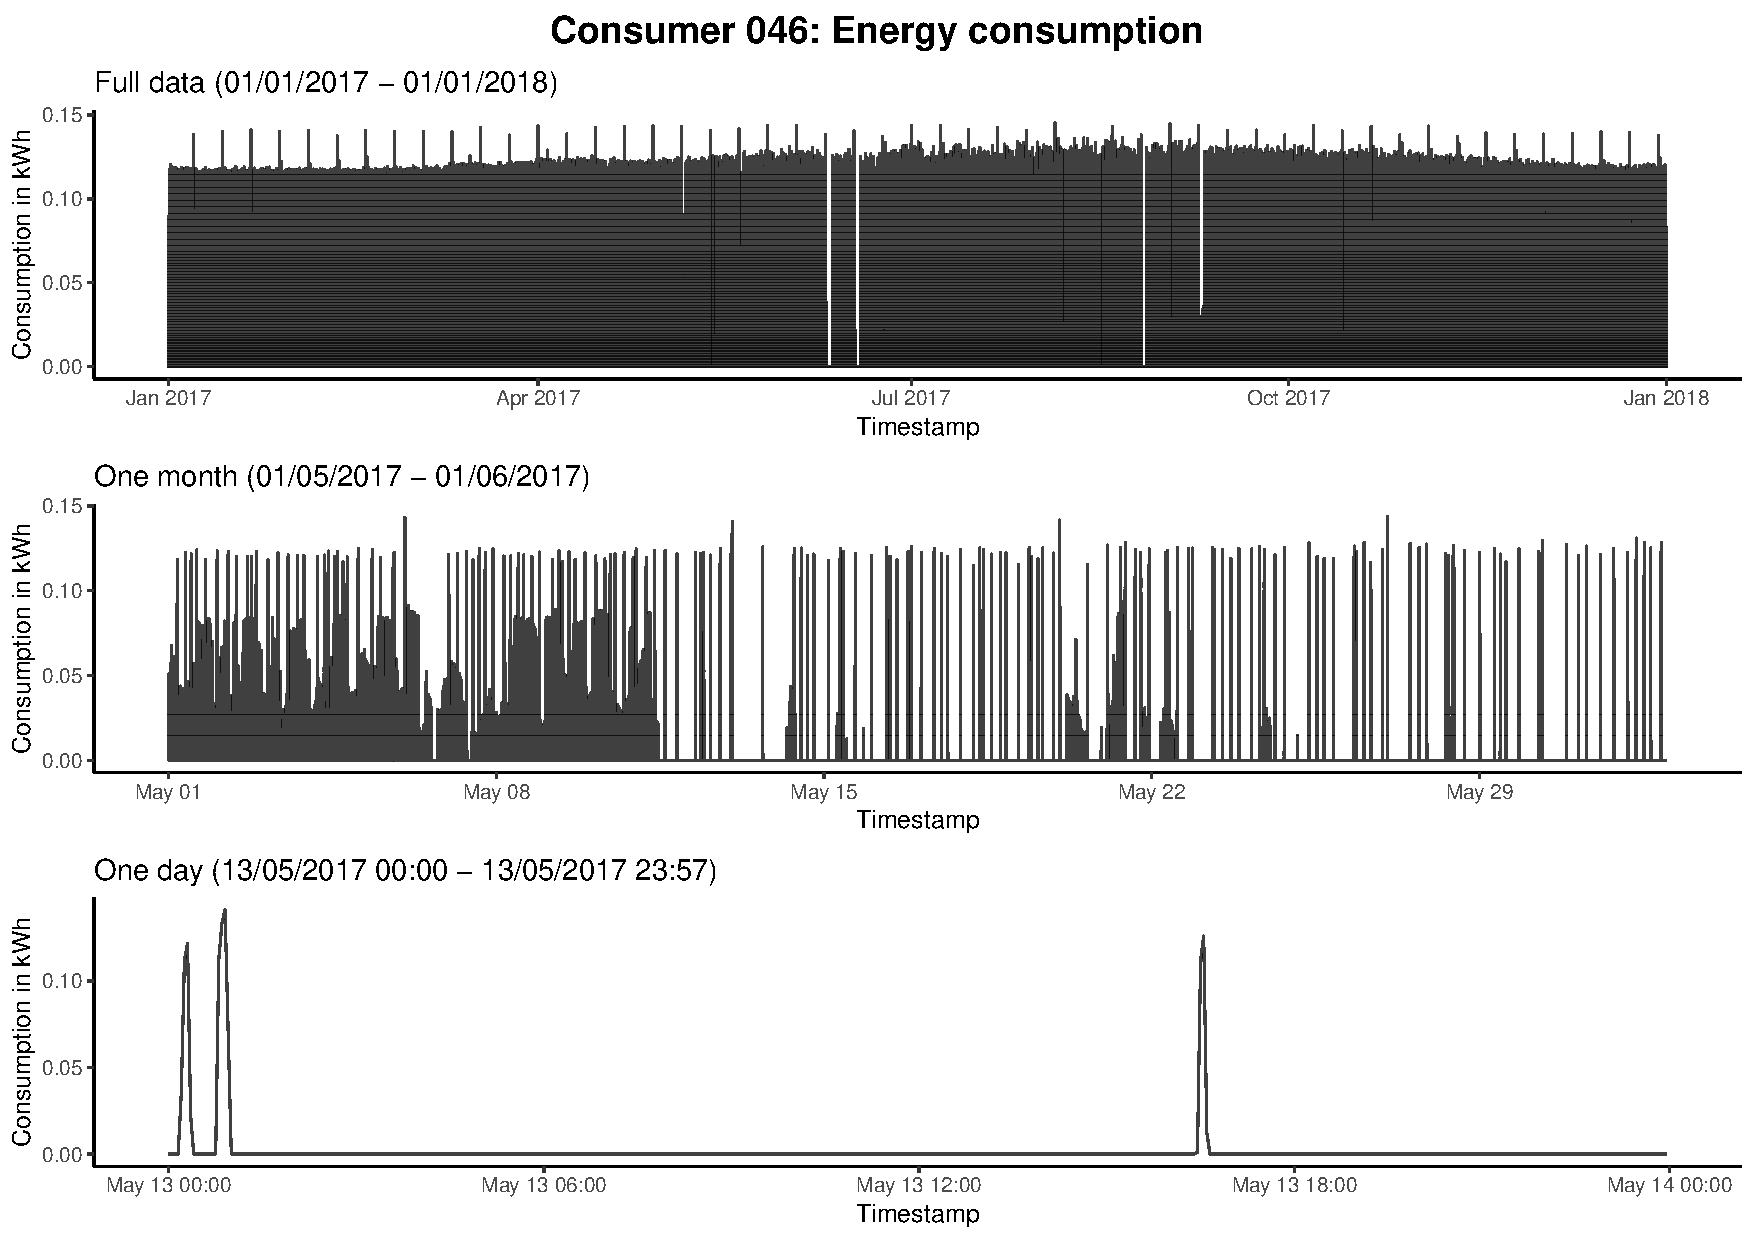
\includegraphics[width=\textwidth-0.85cm]{thesis/graphs/timeseries/c046_cons.pdf}
\end{figure}
\begin{figure}[!htbp]
        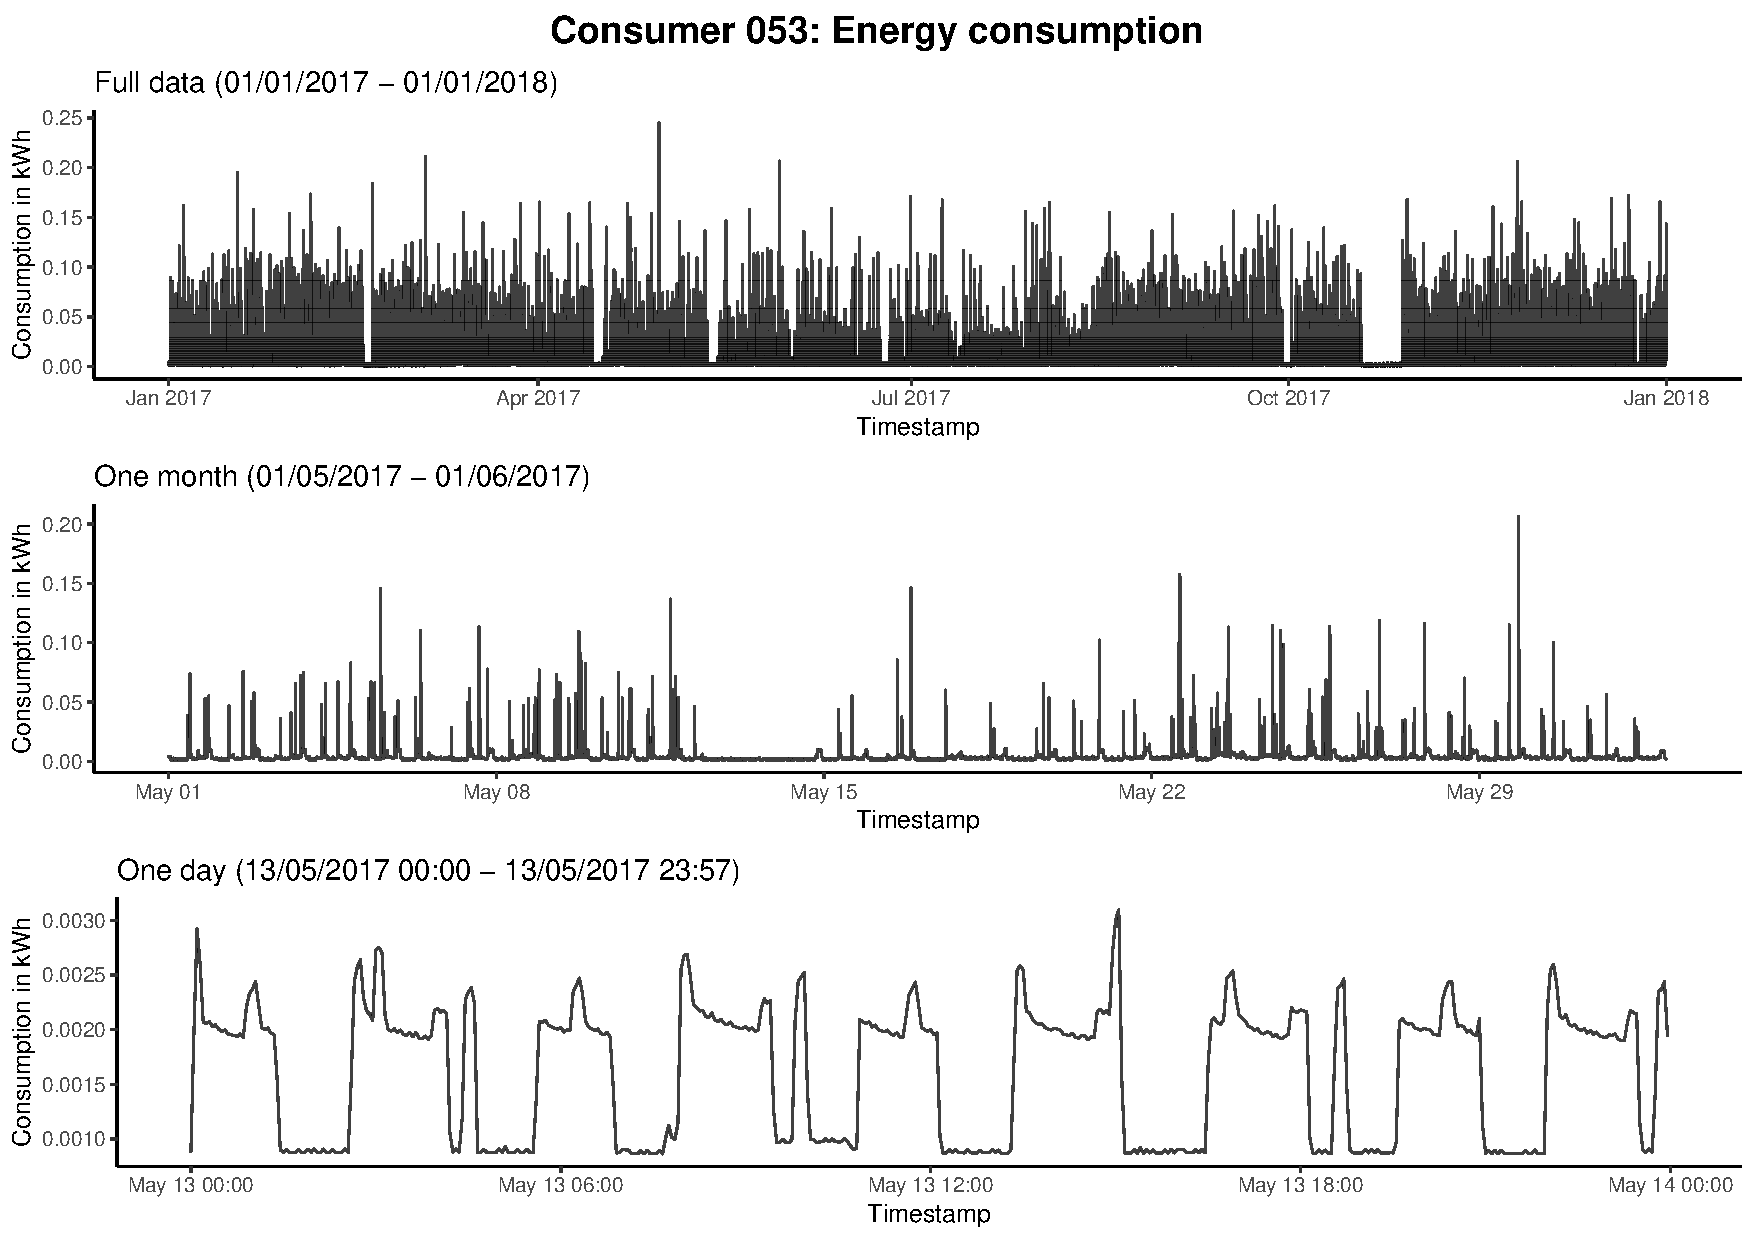
\includegraphics[width=\textwidth-0.85cm]{thesis/graphs/timeseries/c053_cons.pdf}\vspace{0.3cm}
        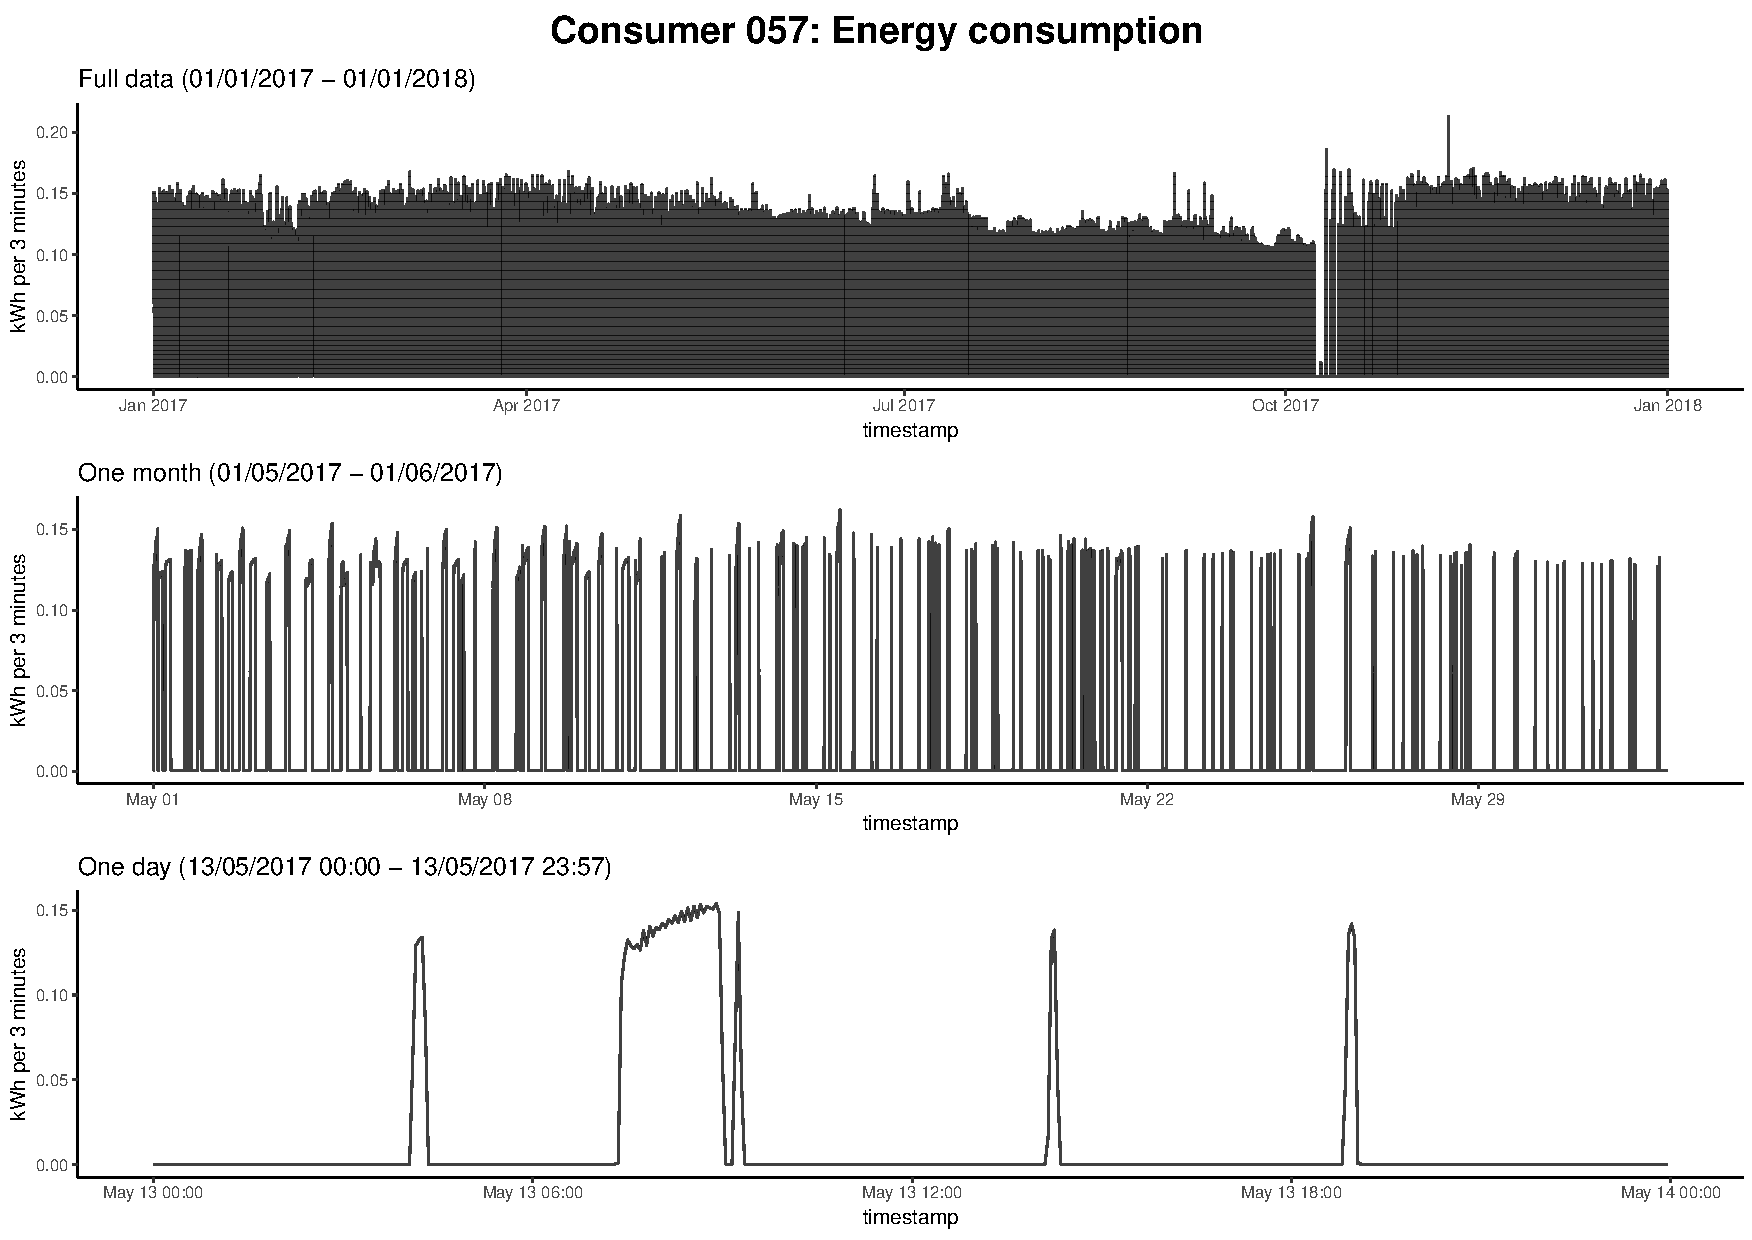
\includegraphics[width=\textwidth-0.85cm]{thesis/graphs/timeseries/c057_cons.pdf}
\end{figure}
\begin{figure}[!htbp]
        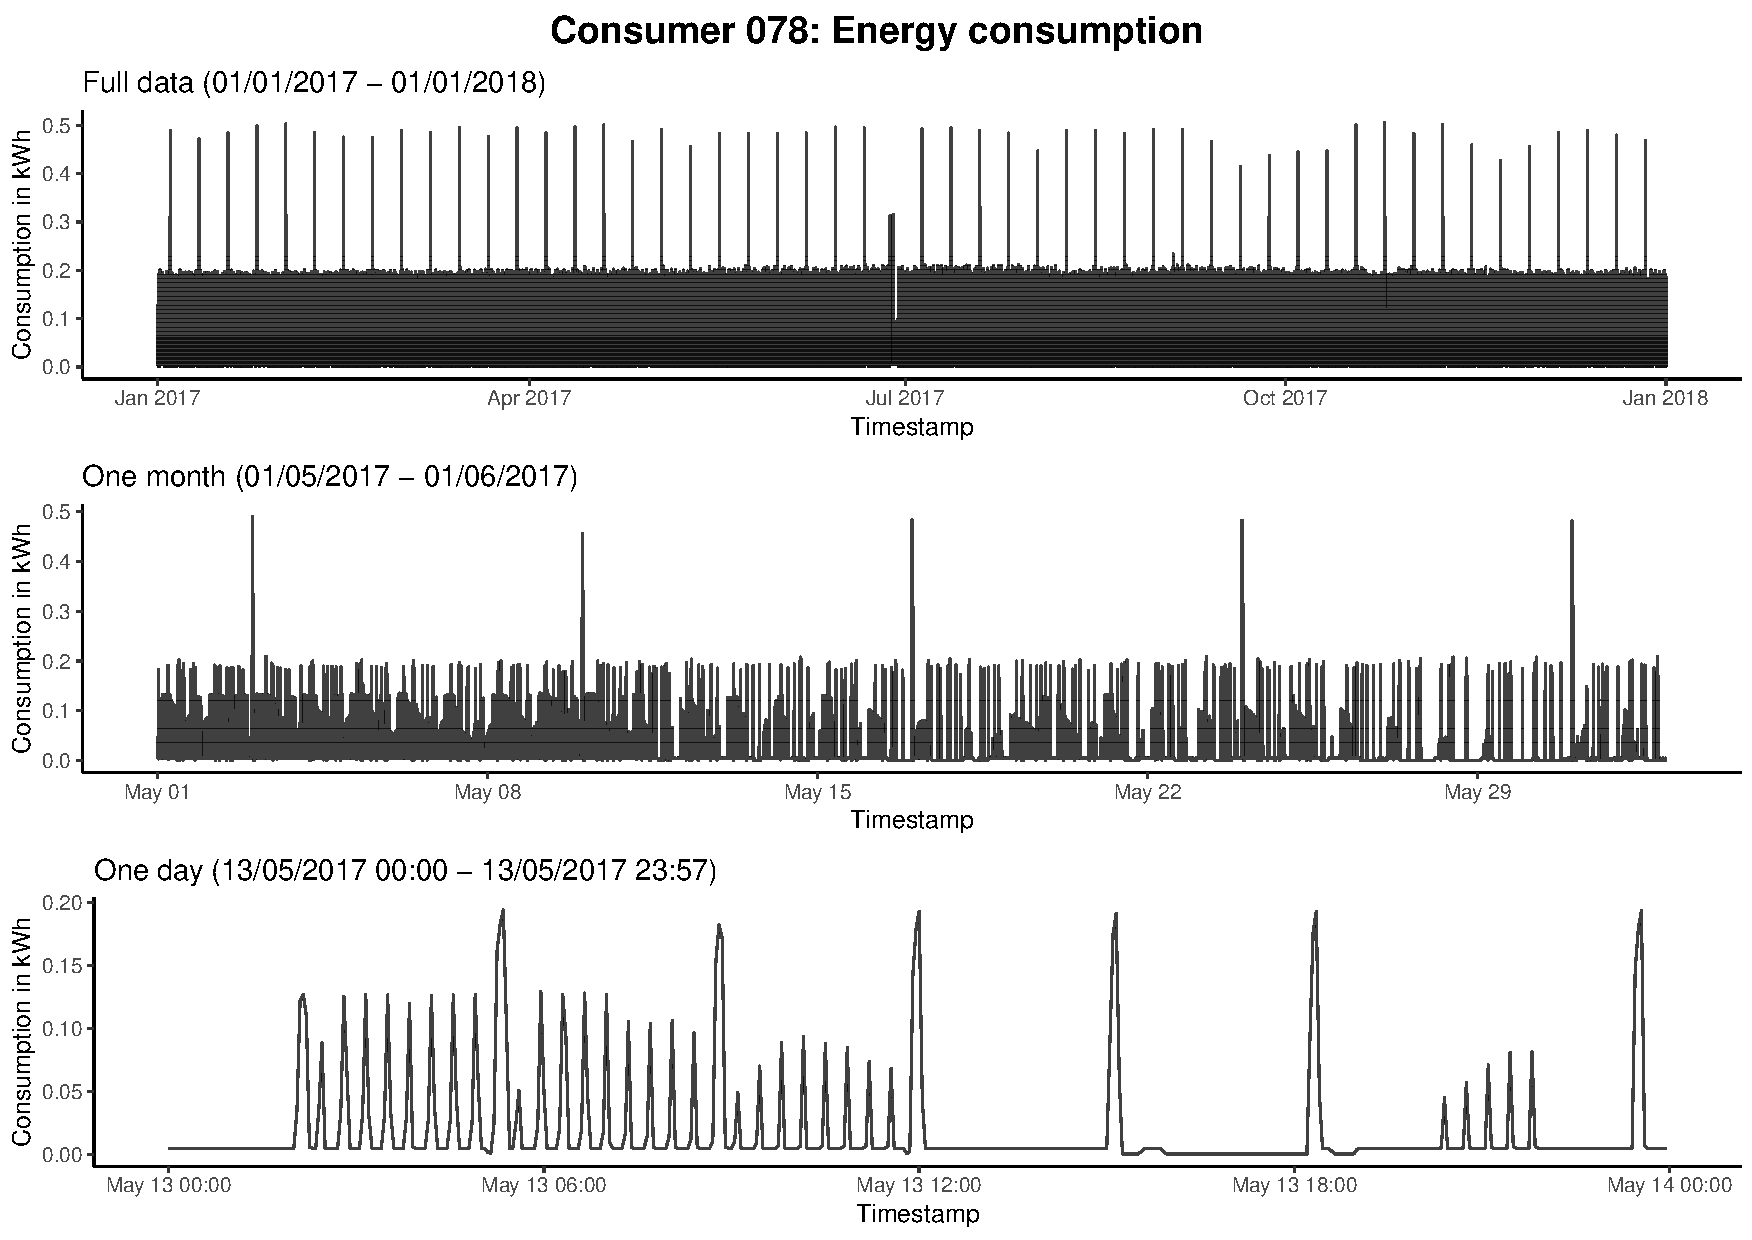
\includegraphics[width=\textwidth-0.85cm]{thesis/graphs/timeseries/c078_cons.pdf}\vspace{0.3cm}
        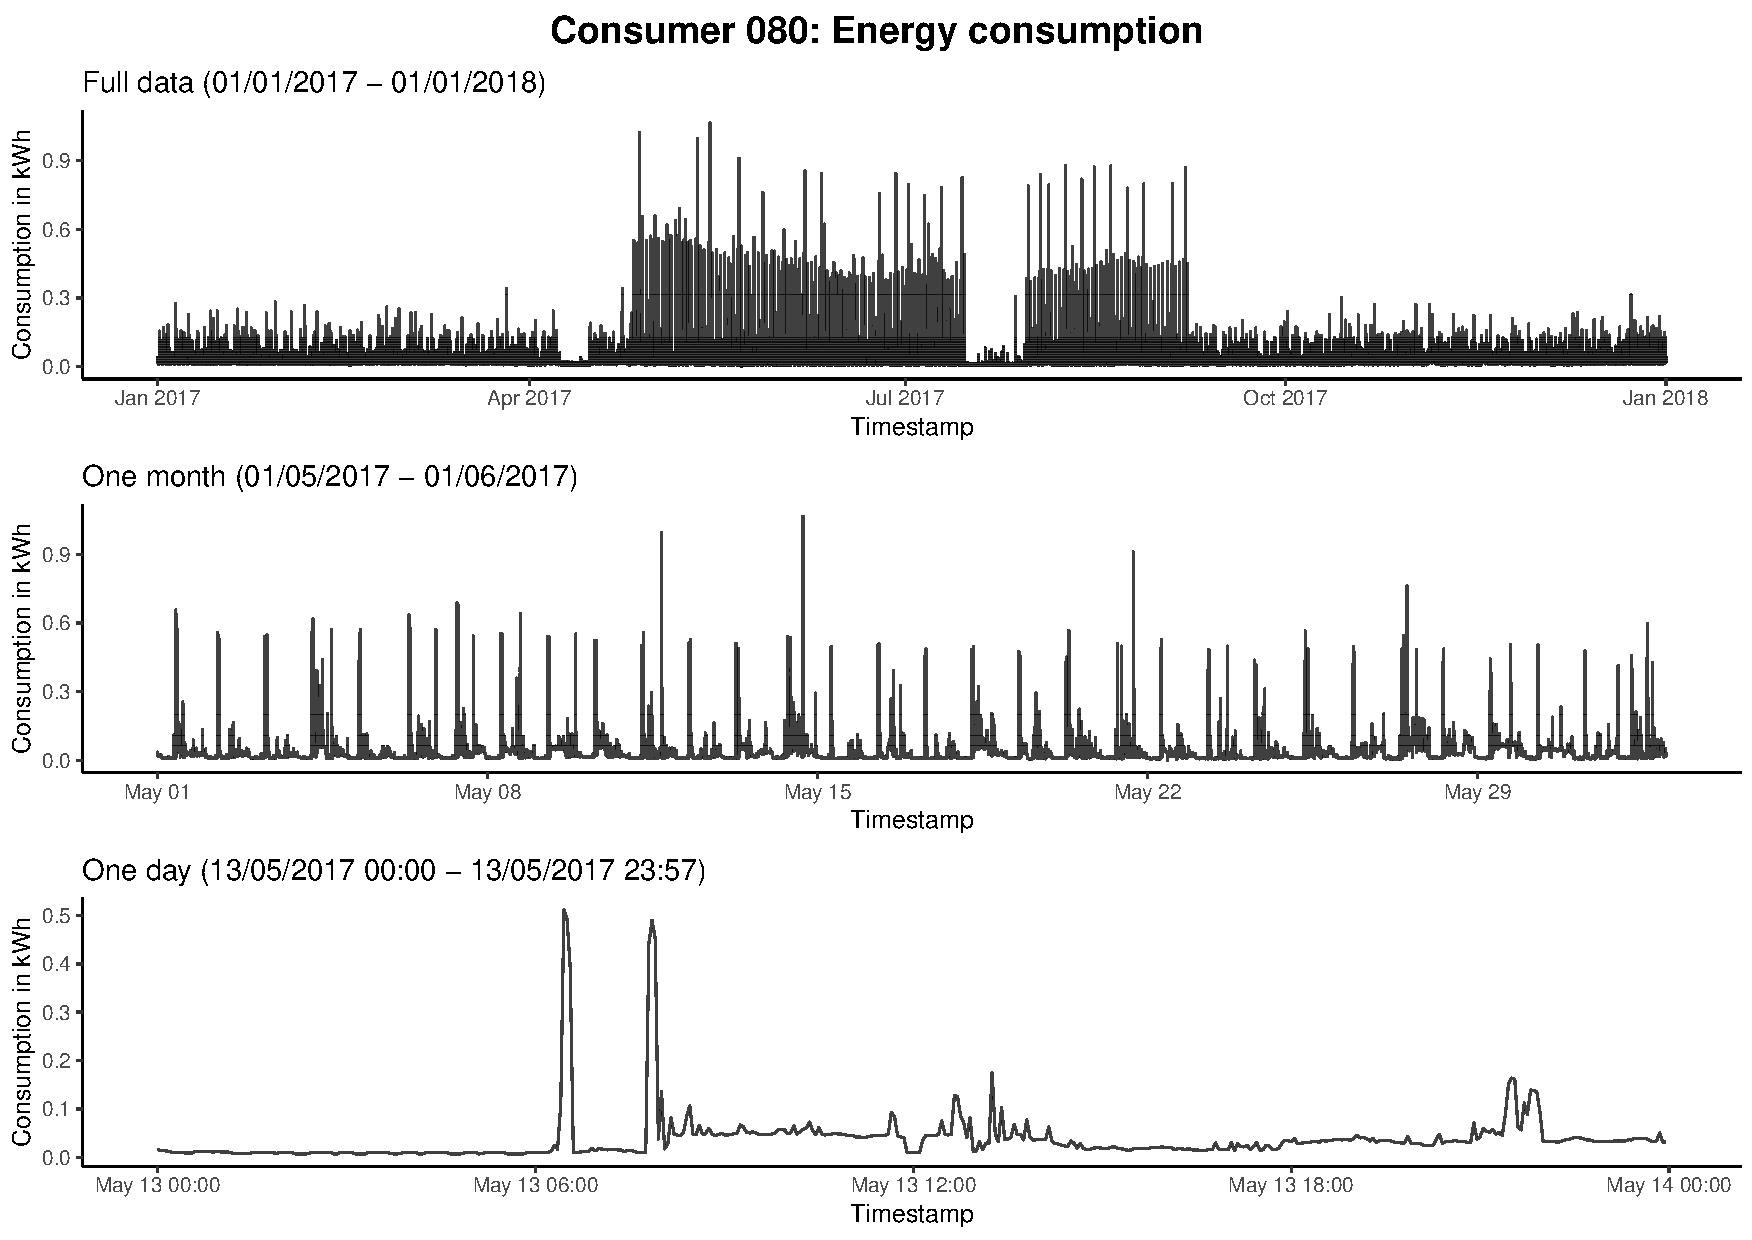
\includegraphics[width=\textwidth-0.85cm]{thesis/graphs/timeseries/c080_cons.pdf}
        \caption[Consumer data sets excluded due to peculiarities in the consumption patterns]{Consumer data sets excluded due to peculiarities in the consumption patterns. \quantnet\href{ }{BLEMplotEnergyData}}
\end{figure}
\end{centering}


\subsection*{\hypertarget{AppA2:Figures:Excludedp}{A2} Excluded consumer data sets}\label{AppA2:Figures:Excludedp}

\begin{centering}
\begin{figure}[H]
        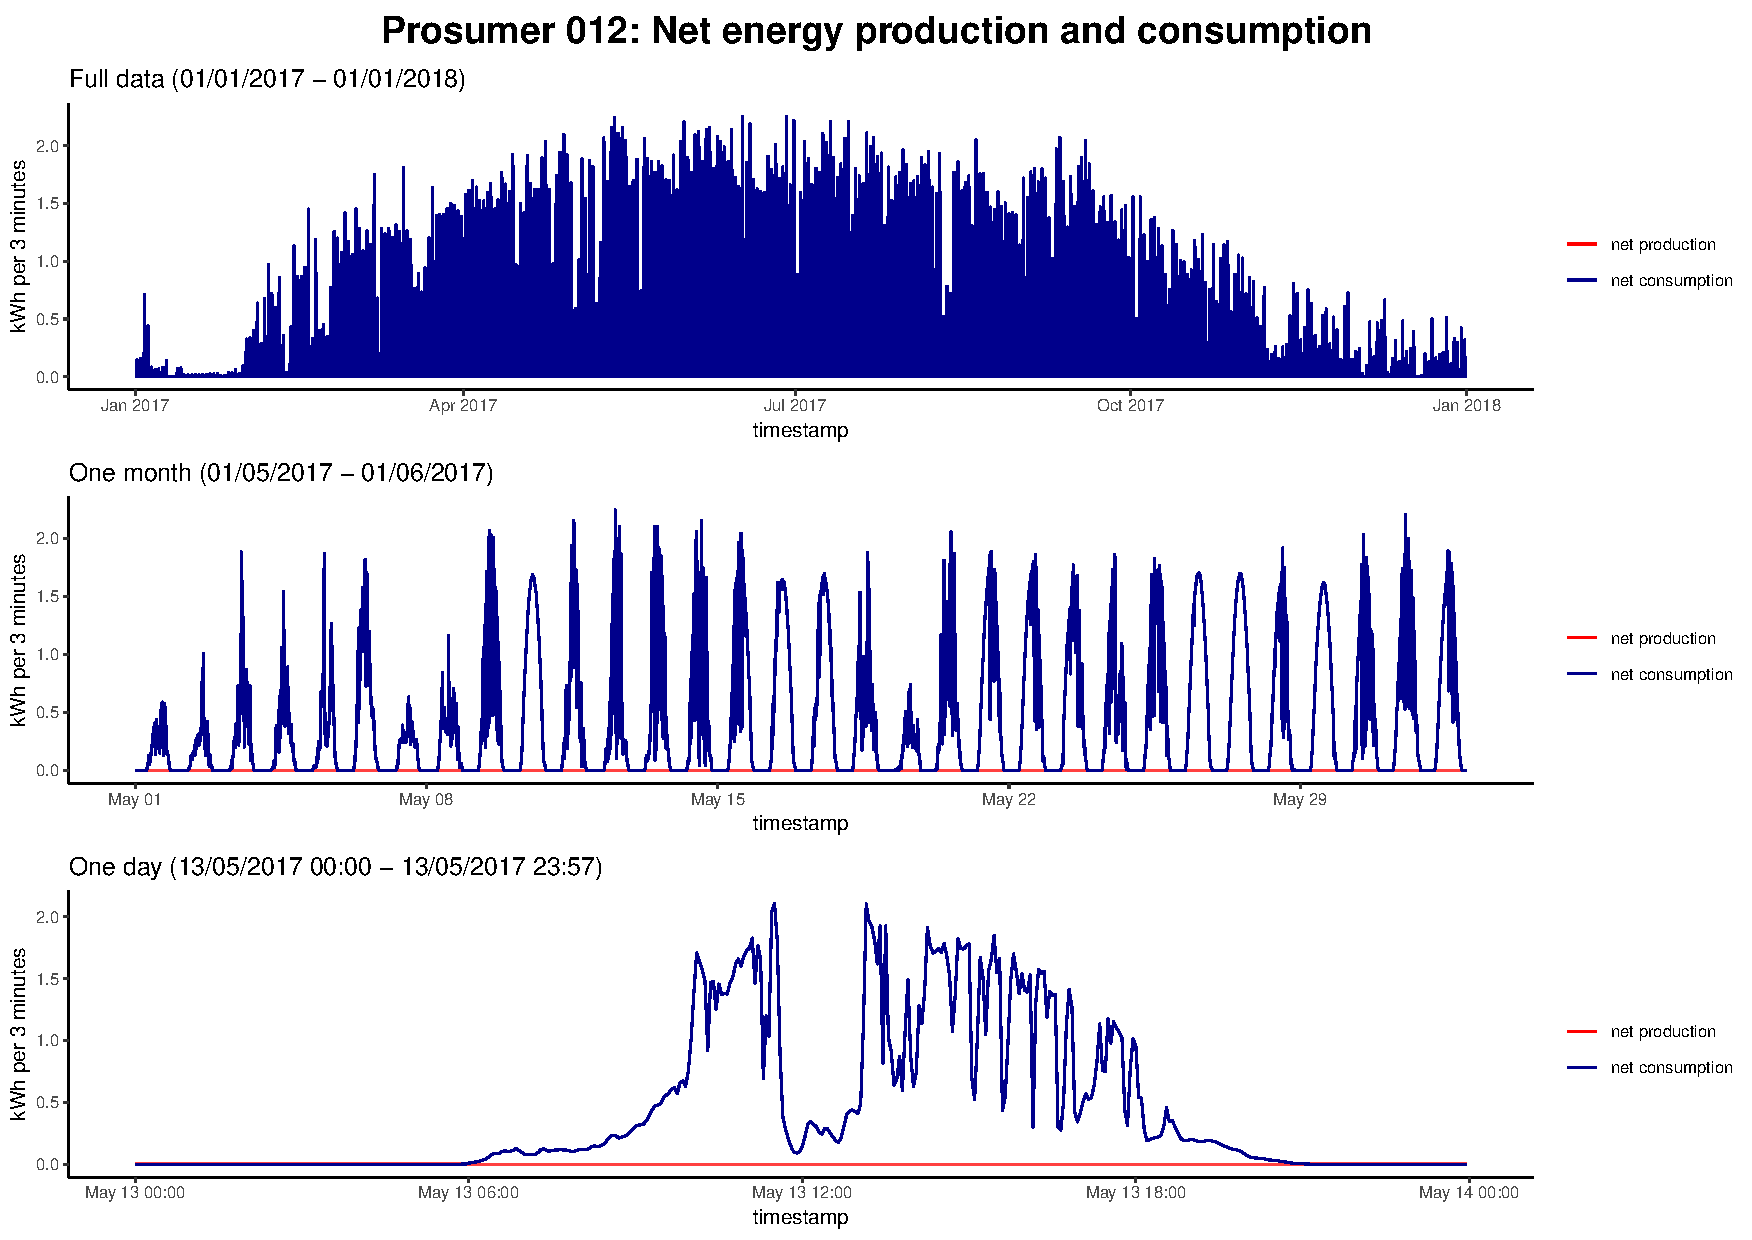
\includegraphics[width=\textwidth-0.85cm]{thesis/graphs/timeseries/p012_prod&cons.pdf}\vspace{0.3cm}
        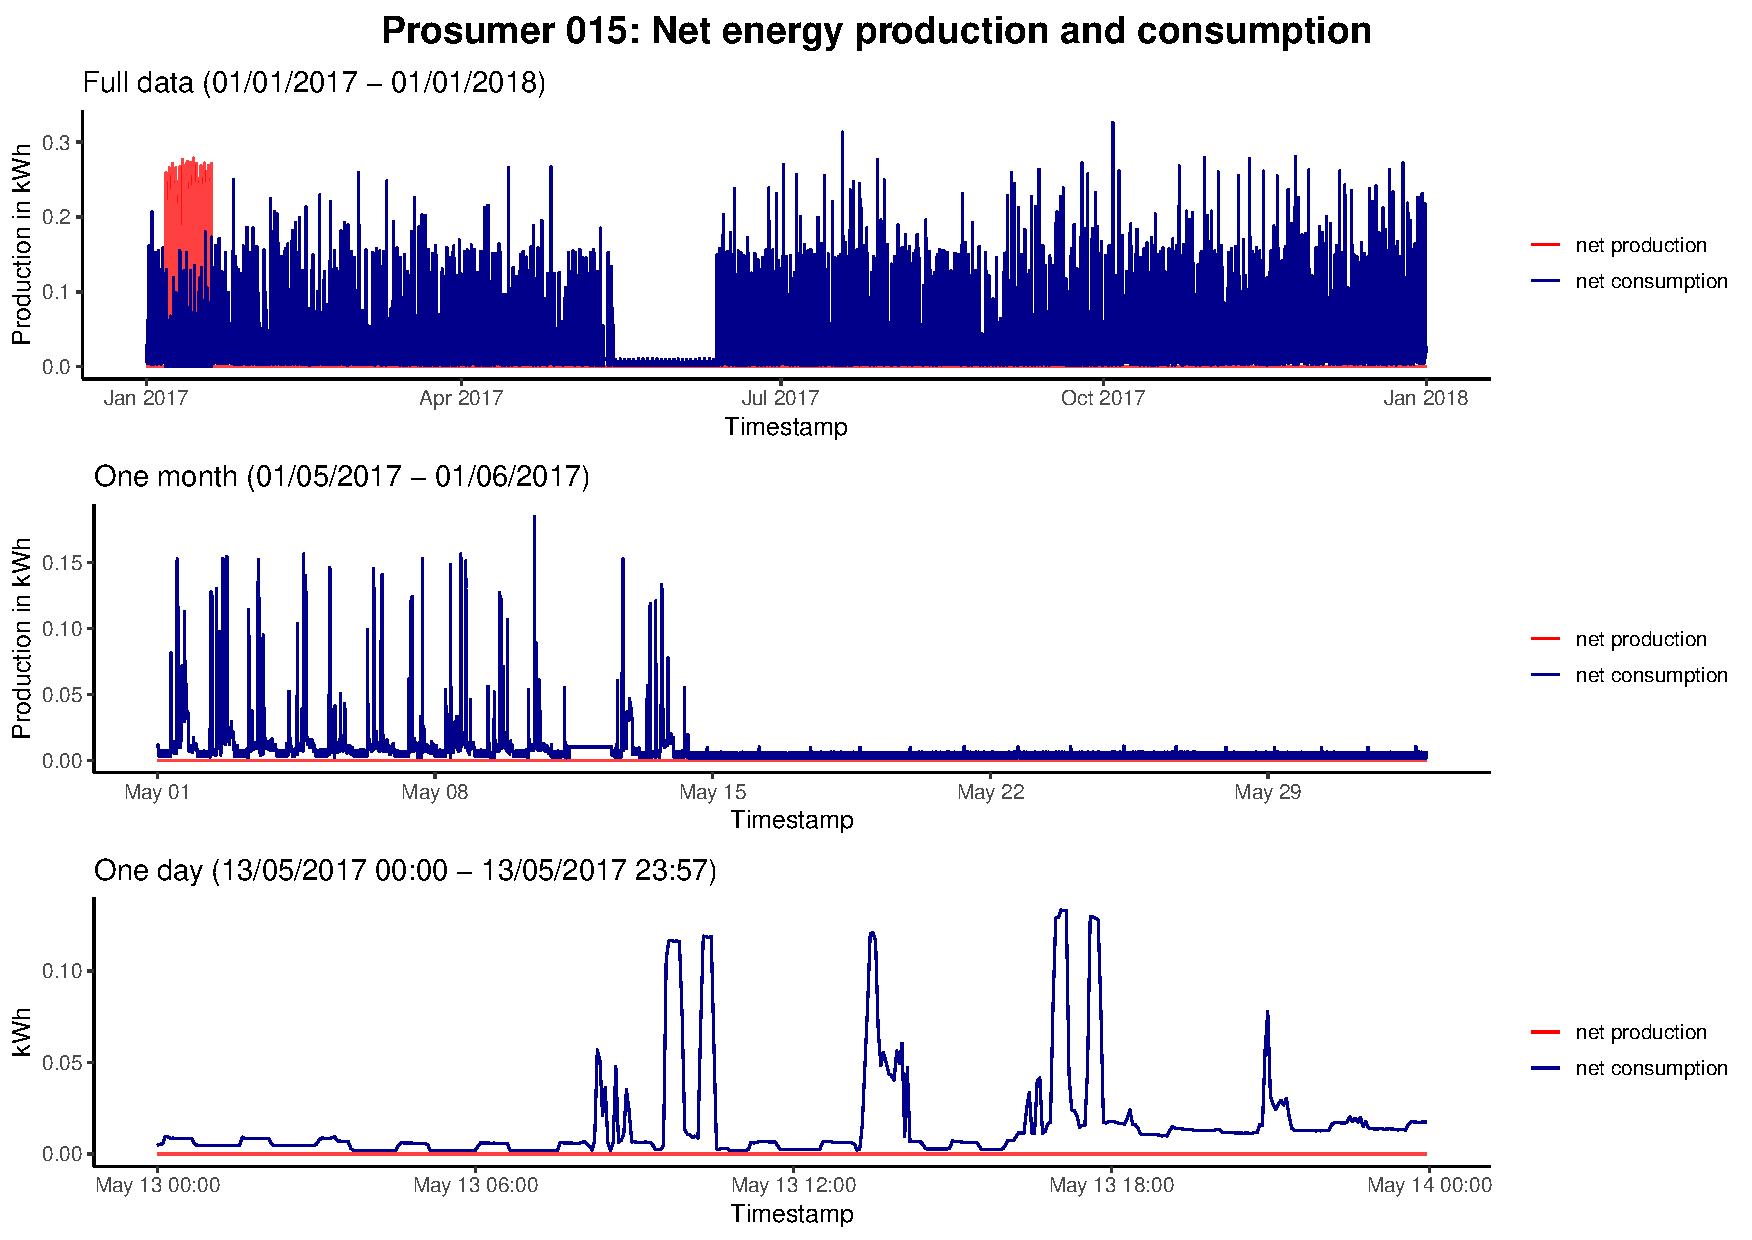
\includegraphics[width=\textwidth-0.85cm]{thesis/graphs/timeseries/p015_prod&cons.pdf}
        \caption[Prosumer data sets excluded due to peculiarities in the consumption patterns]{Prosumer data sets excluded due to peculiarities in the consumption patterns. \quantnet\href{ }{BLEMplotEnergyData}}
\end{figure}
\end{centering}


\subsection*{\hypertarget{AppA3:Figures:transform}{A3} Normalized log-consumption data}\label{AppA3:Figures:transform}

\begin{centering}
\begin{figure}[!htbp]
        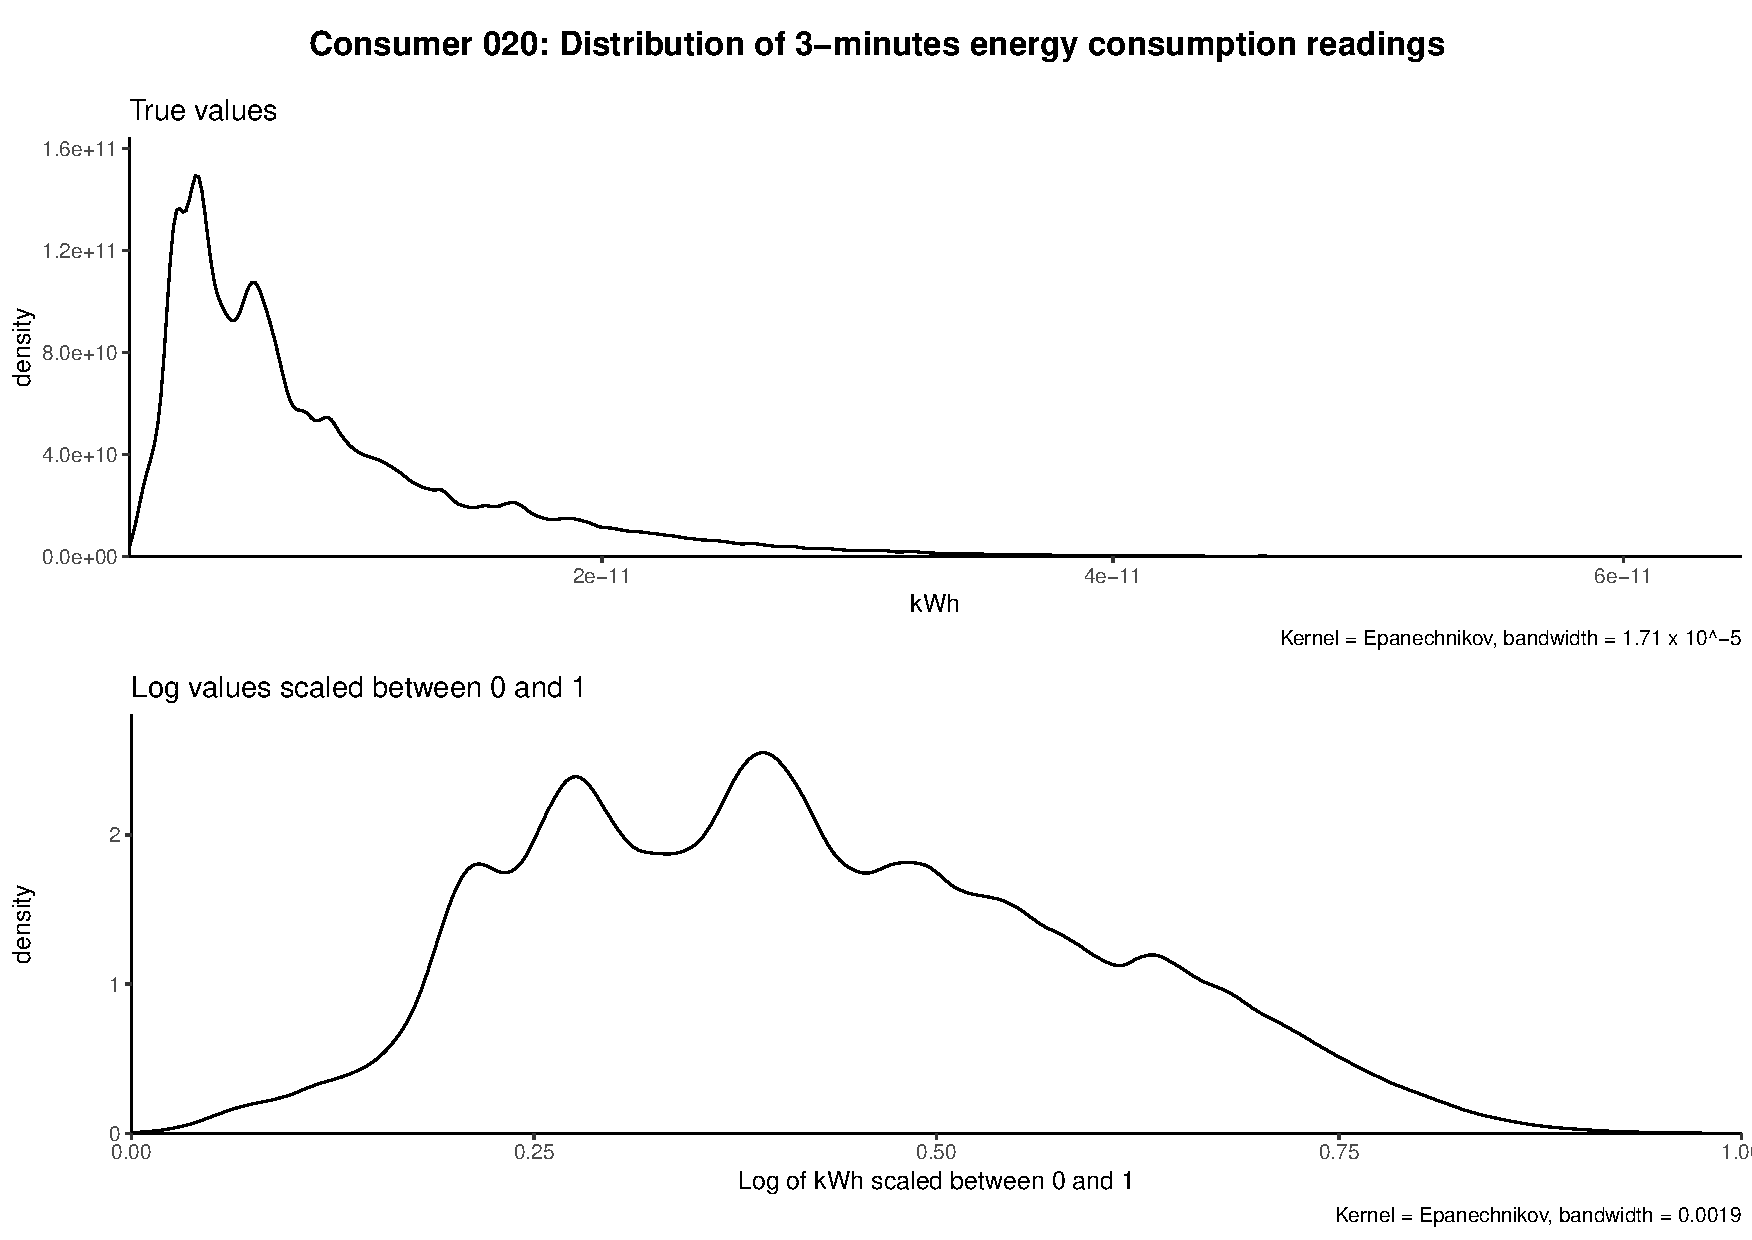
\includegraphics[width=\textwidth-0.85cm]{thesis/graphs/c020_density.pdf}
        \caption[Energy consumption distribution before and after transformation]{Consumer 020's density estimate of energy consumption values before and after transformation. \quantnet\href{ }{BLEMplotScaling}}
\end{figure}
\end{centering}

% \newpage
% \subsection*{\hypertarget{AppA4:Figures:heatmaps}{A4} Heatmaps of error measures}\label{AppA4:Figures:heatmaps}

% \begin{centering}
% \begin{figure}[H]
%     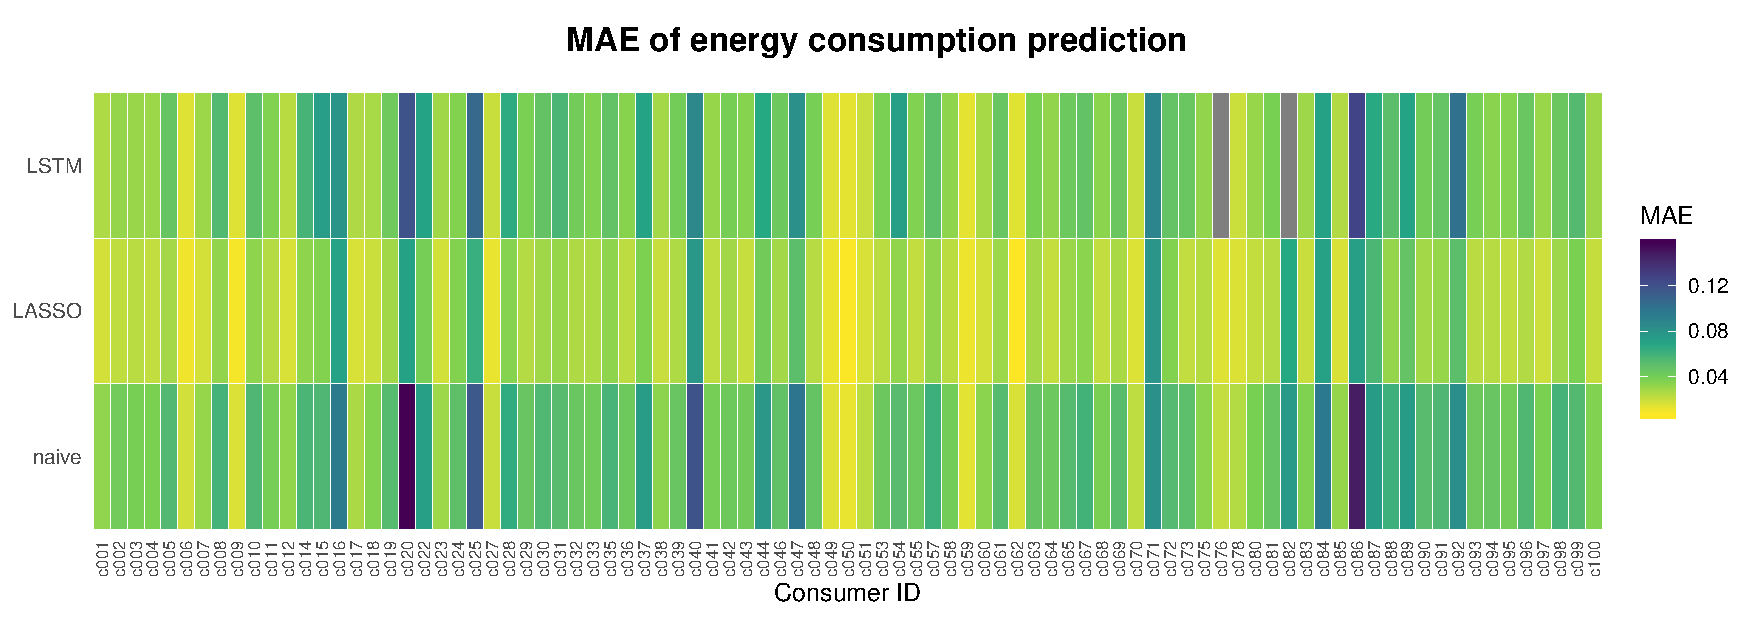
\includegraphics[width=\textwidth]{thesis/graphs/evaluation/c_heatmap_MAE.pdf}
%     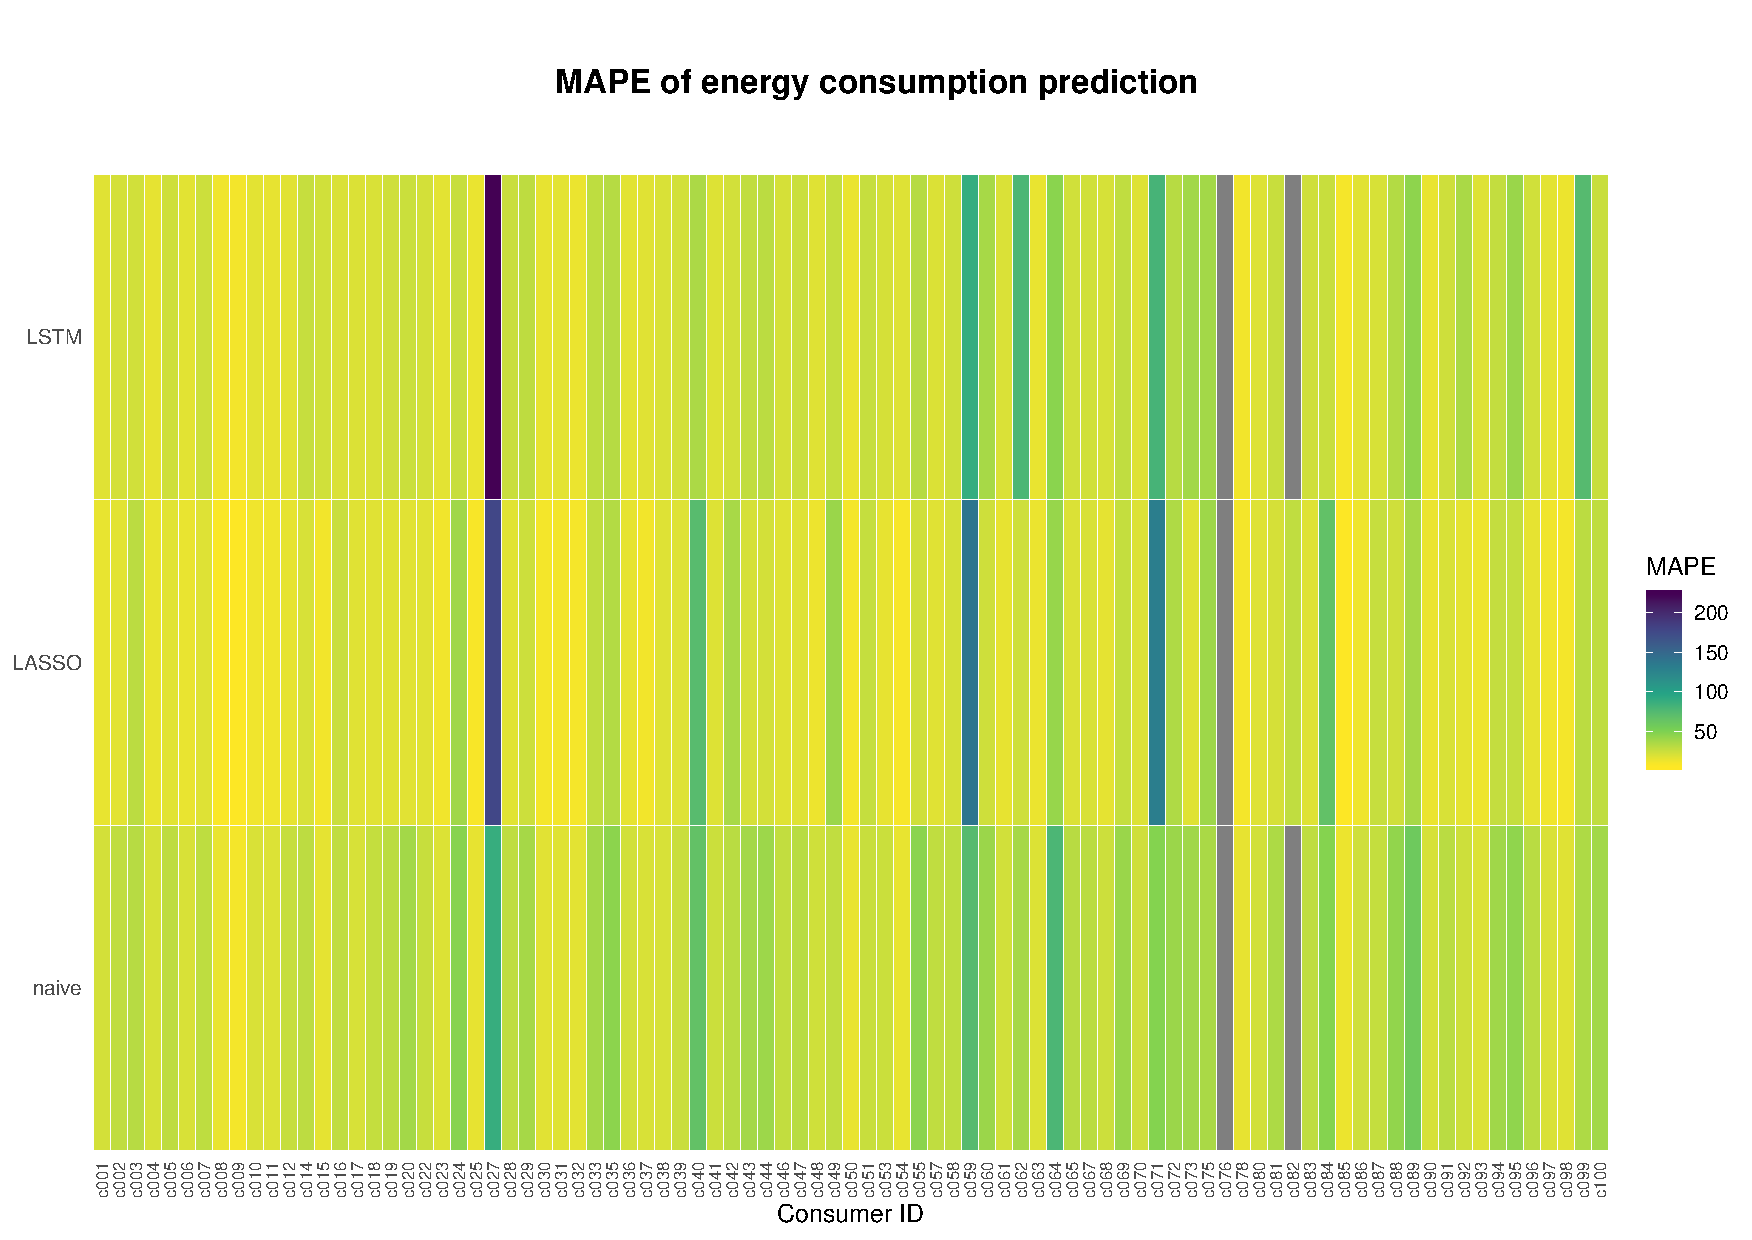
\includegraphics[width=\textwidth]{thesis/graphs/evaluation/c_heatmap_MAPE.pdf}
% \end{figure}
% \begin{figure}[H]
%      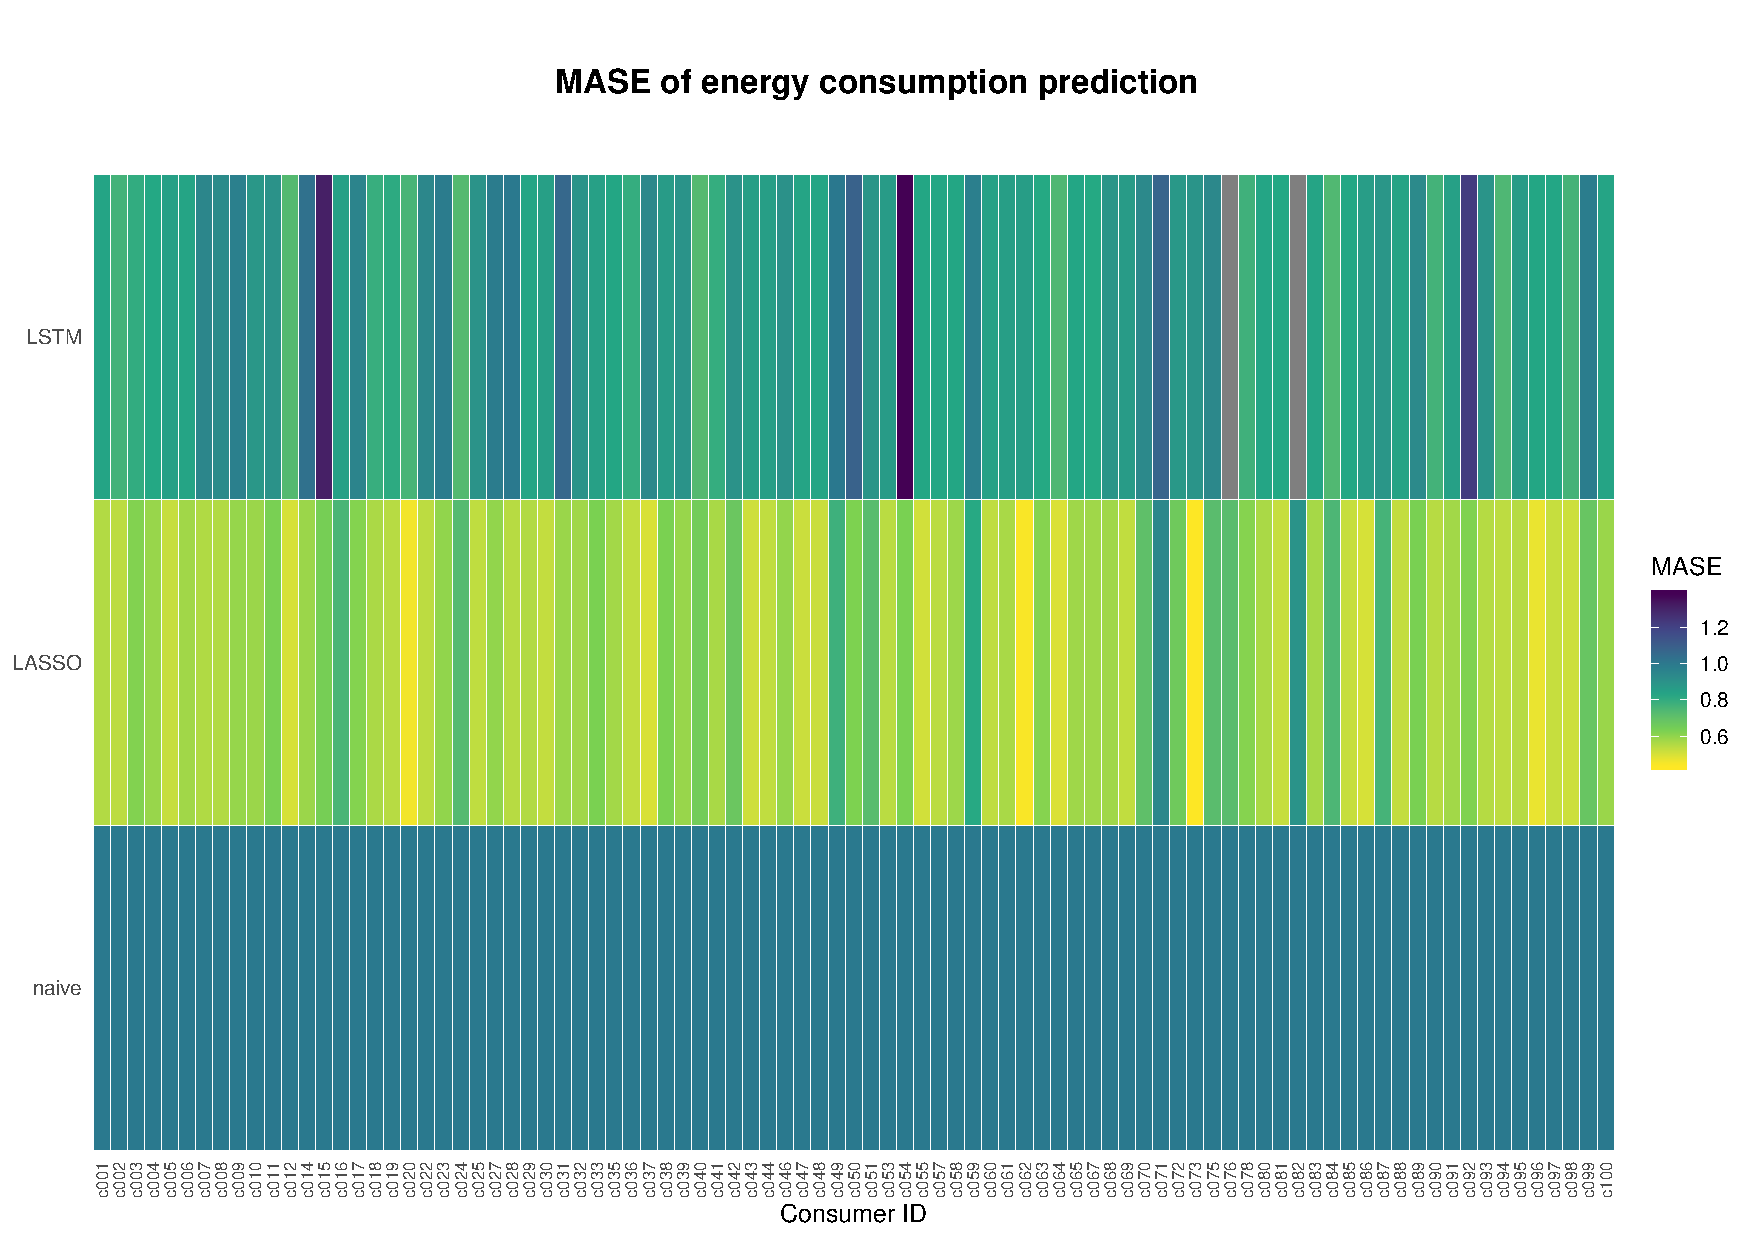
\includegraphics[width=\textwidth]{thesis/graphs/evaluation/c_heatmap_MASE.pdf}
%      \caption[Heatmaps of MAE, MAPE, and MASE scores for the prediction of consumption values]{Heatmaps of MAE, MAPE, and MASE scores for the prediction of consumption values per consumer data set. \quantnet }
% \end{figure}
% \end{centering}


\subsection*{\hypertarget{AppA4:Figures:erroranalysis}{A4} Error analysis of consumer 027}\label{AppA4:Figures:erroranalysis}

\begin{centering}
\begin{figure}[H]
    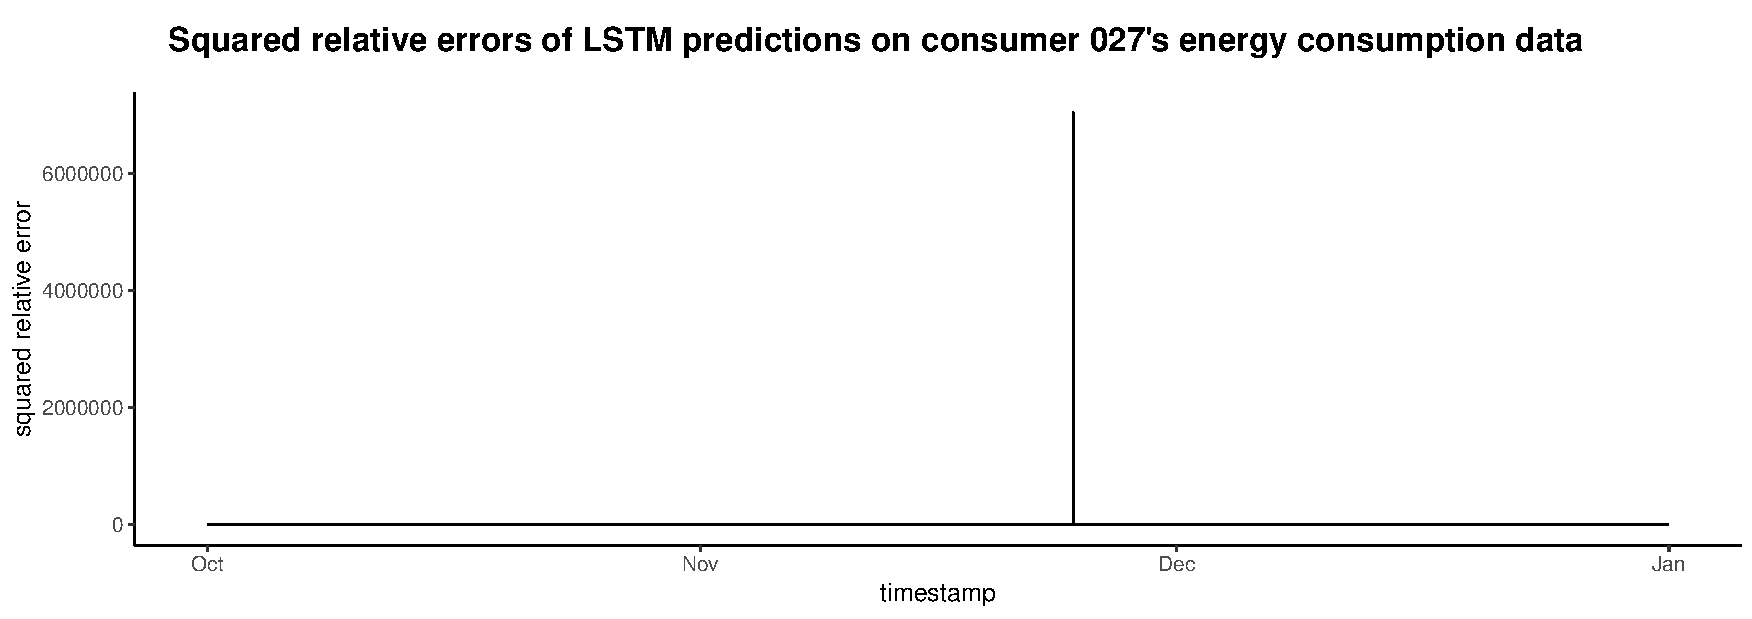
\includegraphics[width=\textwidth]{thesis/graphs/evaluation/c027_squarederrors.pdf}
    \caption[Squared relative errors of predictions by LSTM model on consumer 027]{Squared relative errors of predictions by LSTM model on data set of consumer 027. \quantnet\href{ }{}}
\end{figure}
\end{centering}


%%%%%%%%%%%%%%%%%%%%%%%%%%%%%%%%%%%%%%%%%%%%%%%%%%%%%%%%%%%%
